% This is text associated with the open textbook "Open Electromagnetics"
% See immediately below for author, date
% This work is licensed under the Creative Commons Attribution-ShareAlike 4.0 International License. (CC BY SA 4.0) 
% To view a copy of the license, visit http://creativecommons.org/licenses/by-sa/4.0/

%ORB TITLE Wave Polarization
%ORB AUTHOR 0        # S.W. Ellingson, Virginia Tech (ellingson@vt.edu)
%ORB DATE 20180807   # yyyymmdd
%ORB ABSTRACT Wave Polarization

\label{m0131_Wave_Polarization} % <-- Must match name of this file and module directory name.  Don't mess with this!
\index{polarization|}
\index{waves!polarization|(}

\emph{Polarization} refers to the orientation of the electric field vector.
For waves, the term ``polarization'' refers specifically to the orientation of this vector with increasing distance along the direction of propagation, or, equivalently, the orientation of this vector with increasing time at a fixed point in space.
The relevant concepts are readily demonstrated for uniform plane waves, as shown in this section.
A review of Section~\ref{m0039_Uniform_Plane_Waves_Characteristics} (``Uniform Plane Waves: Characteristics'') is recommended before reading further.

To begin, consider the following uniform plane wave, described in terms of the phasor representation of its electric field intensity:
%
\begin{equation}
\widetilde{\bf E}_x = \hat{\bf x}E_x e^{-j\beta z}
\end{equation}
%
Here $E_x$ is a complex-valued constant representing the magnitude and phase of the wave,
and $\beta$ is the positive real-valued propagation constant.  
Therefore, this wave is propagating in the $+\hat{\bf z}$ direction in lossless media.
This wave is said to exhibit \emph{linear} polarization 
\index{polarization!linear}
(and ``linearly polarized'')
 because the electric field always points in the same direction, namely $+\hat{\bf x}$.
Now consider the wave
%
\begin{equation}
\widetilde{\bf E}_y = \hat{\bf y}E_y e^{-j\beta z}
\end{equation}
%
Note that $\widetilde{\bf E}_y$ is identical to $\widetilde{\bf E}_x$ except that the electric field vector now points in the $+\hat{\bf y}$ direction and has magnitude and phase that is different by the factor $E_y/E_x$.
This wave too is said to exhibit linear polarization, because, again, the direction of the electric field is constant with both time and position.
In fact, \emph{all} linearly-polarized uniform plane waves propagating in the $+\hat{\bf z}$ direction in lossless media can be described as follows:
%
\begin{equation}
\widetilde{\bf E} = \hat{\bf \rho}E_{\rho} e^{-j\beta z}
\end{equation}
%
This is so because $\hat{\bf \rho}$ could be $\hat{\bf x}$, $\hat{\bf y}$, or any other direction that is perpendicular to $\hat{\bf z}$.
If one is determined to use Cartesian coordinates, the above expression may be rewritten using (Section~\ref{m0096_Cylindrical_Coordinates})
%
\begin{equation}
\hat{\bf \rho} = \hat{\bf x}\cos\phi + \hat{\bf y}\cos\phi
\end{equation}
%
yielding
%
\begin{equation}
\widetilde{\bf E} = \left( \hat{\bf x}\cos\phi + \hat{\bf y}\cos\phi \right) E_{\rho} e^{-j\beta z}
\label{m0131_eLinAI}
\end{equation}
%
When written in this form, 
$\phi=0$ corresponds to $\widetilde{\bf E}=\widetilde{\bf E}_x$,
$\phi=\pi/2$ corresponds to $\widetilde{\bf E}=\widetilde{\bf E}_y$,
and any other value of $\phi$ corresponds to some other constant orientation of the electric field vector;
see Figure~\ref{m0131_fLinearly_Polarized_Wave} for an example.
%
\begin{figure}
\begin{center}
\pdftooltip{{  % note double braces
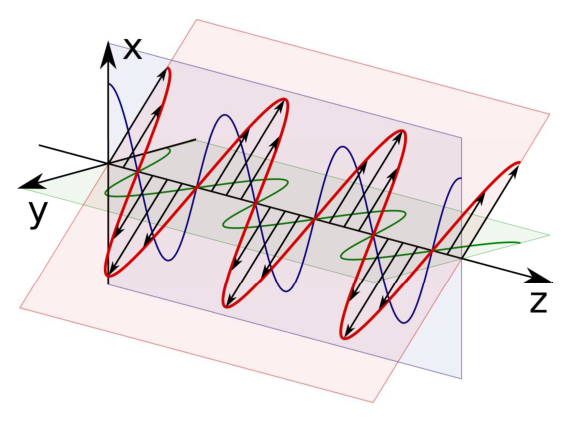
\includegraphics[width=\columnwidth]{modules/m0131_Linearly_Polarized_Wave.eps}
% https://commons.wikimedia.org/wiki/File:Linearly_Polarized_Wave.svg
}}{Similar to a previous figure. Cartesian coordinates with x (vertical), y (out-of-page), and z (horizontal) axes. A sinusoidal wave (blue) with a maximum at the x-intercept extends down the z-axis. Perpendicular to the first wave, the a second sinusoid (green) is in the y-z plane. At an angle phi equals pi over 4, sits a red plane, where the sinusoidal wave travels the length of the z axis at the angle phi. For both the red and green waves vectors point from the z-axis to the waveform.}
\end{center} 
\centerline{\scriptsize 
by~\hyperref[m0131_Linearly_Polarized_Wave_Credit]{RJB1} (Modified) 
} 
\caption{
\label{m0131_fLinearly_Polarized_Wave}
Linear polarization.  Here ${\bf E}_x$ is shown in blue, ${\bf E}_y$ is shown in green, and ${\bf E}$ is shown in red with black vector symbols.  In this example the phases of $E_x$ and $E_y$ are zero and $\phi=-\pi/4$.
}
\end{figure}


%ORB HIGHLIGHT
\begin{mdframed}[backgroundcolor=yellow!20,nobreak=true] 
A wave is said to exhibit linear polarization if the direction of the electric field vector does not vary with either time or position.
\end{mdframed}

Linear polarization arises when the source of the wave is linearly polarized.  
A common example is the wave radiated by a straight wire antenna, 
\index{antenna}
such as a dipole 
\index{antenna!dipole}
\index{dipole|see{antenna}}
or a monopole.
\index{antenna!monopole}
\index{monopole|see{antenna}}
Linear polarization may also be created by passing a plane wave through a \emph{polarizer}; 
\index{polarizer}
this is particularly common at optical frequencies (see ``Additional Reading'' at the end of this section).

A commonly-encountered alternative to linear polarization is \emph{circular polarization}.
\index{polarization!circular}
For an explanation, let us return to the linearly-polarized plane waves $\widetilde{\bf E}_x$ and $\widetilde{\bf E}_y$ defined earlier.
If both of these waves exist simultaneously, then the total electric field intensity is simply the sum:
%  
\begin{flalign}
\widetilde{\bf E} &= \widetilde{\bf E}_x +\widetilde{\bf E}_y  \nonumber \\
                  &= \left( \hat{\bf x}E_x + \hat{\bf y}E_y \right) e^{-j\beta z}  
\label{m0131_eCirc1}
\end{flalign}
%
If the phase of $E_x$ and $E_y$ is the same, then $E_x = E_{\rho}\cos\phi$, $E_y = E_{\rho}\sin\phi$, and the above expression is essentially the same as Equation~\ref{m0131_eLinAI}.
In this case, $\widetilde{\bf E}$ is linearly polarized.
But what if the phases of $E_x$ and $E_y$ are different?
In particular, let's consider the following case. Let $E_x = E_0$, some complex-valued constant, and let $E_y = +jE_0$, which is $E_0$ phase-shifted by $+\pi/2$ radians. 
With no further math, it is apparent that $\widetilde{\bf E}_x$ and $\widetilde{\bf E}_y$ are different only in that one is phase-shifted by $\pi/2$ radians relative to the other.
For the physical (real-valued) fields, this means that ${\bf E}_x$ has maximum magnitude when ${\bf E}_y$ is zero and vice versa.
As a result, the direction of ${\bf E}={\bf E}_x+{\bf E}_y$ will rotate in the $x-y$ plane, as shown in Figure~\ref{m0131_fCircular_Polarized_Wave}
%
\begin{figure}
\begin{center}
\pdftooltip{{  % note double braces
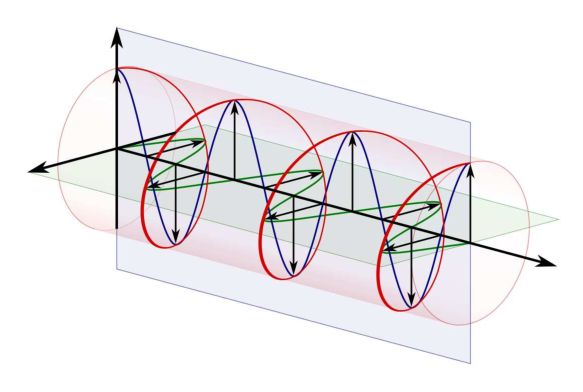
\includegraphics[width=\columnwidth]{modules/m0131_Circular.Polarization.Circularly.Polarized.Light_With.Components_Left.Handed.eps}
% https://en.wikipedia.org/wiki/File:Circular.Polarization.Circularly.Polarized.Light_With.Components_Left.Handed.svg
}}{Similar to a previous figure, except the xyz coordinates show only the blue and green planes and waves. Black vectors extend from the z-axis to the top of the waves in the blue and green planes. A red path connects the peaks of each wave in a circular manner as it travels the z-axis. The final image looks like a coil of wire with a vertical and horizontal sinusoidal wave inside it.}
\end{center} 
\centerline{\scriptsize 
by~\hyperref[m0131_Circular.Polarization.Circularly.Polarized.Light_With.Components_Left.Handed_Credit]{Dave3457} 
} 
\caption{
\label{m0131_fCircular_Polarized_Wave}
A circularly-polarized wave (in red, with black vector symbols) resulting from the addition of orthogonal linearly-polarized waves (shown in green and blue) that are phase-shifted by $\pi/2$ radians.
}
\end{figure}

The rotation of the electric field vector can also be identified mathematically.  When $E_x = E_0$ and $E_y = +jE_0$, Equation~\ref{m0131_eCirc1} can be written:
%  
\begin{equation}
\widetilde{\bf E} = \left( \hat{\bf x} + j\hat{\bf y} \right) E_0 e^{-j\beta z}  
\end{equation}
%
Now reverting from phasor 
\index{phasor}
notation to the physical field:
%  
\begin{flalign}
{\bf E} &= \mbox{Re}\left\{ \widetilde{\bf E} e^{j\omega t} \right\} \nonumber \\
        &= \mbox{Re}\left\{ \left( \hat{\bf x} + j\hat{\bf y} \right) E_0 e^{-j\beta z} e^{j\omega t} \right\} \nonumber \\
        &= \hat{\bf x} \left|E_0\right| \cos\left(\omega t - \beta z \right) + \hat{\bf y} \left|E_0\right| \cos\left(\omega t - \beta z +\frac{\pi}{2} \right) 
\end{flalign}
%
As anticipated, we see that both ${\bf E}_x$ and ${\bf E}_y$ vary sinusoidally, but are $\pi/2$ radians out of phase resulting in rotation in the plane perpendicular to the direction of propagation.

In the example above, the electric field vector rotates either clockwise or counter-clockwise relative to the direction of propagation.  The direction of this rotation can be identified by pointing the thumb of the left hand in the direction of propagation; in this case, the fingers of the left hand curl in the direction of rotation.  For this reason, this particular form of circular polarization is known as \emph{left circular} (or ''left-hand'' circular) polarization (LCP).  
If we instead had chosen $E_y = -jE_0 = -jE_x$, then the direction of ${\bf E}$ rotates in the opposite direction, giving rise to \emph{right circular} (or ``right-hand'' circular) polarization (RCP).
These two conditions are illustrated in Figure~\ref{m0131_fLCP-RCP}.
%
\begin{figure}
\begin{center}
\pdftooltip{{  % note double brace
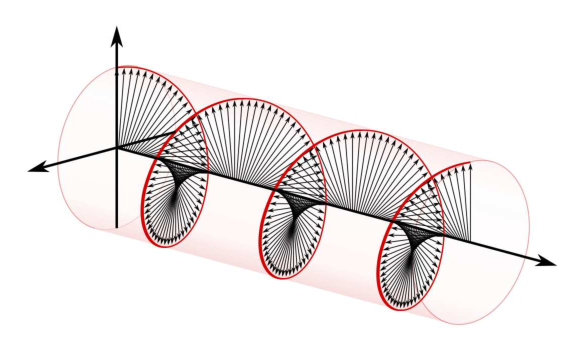
\includegraphics[width=\columnwidth]{modules/m0131_Circular.Polarization.Circularly.Polarized.Light_Without.Components_Left.Handed.eps}
% https://en.wikipedia.org/wiki/File:Circular.Polarization.Circularly.Polarized.Light_Without.Components_Left.Handed.svg
}}{Similar to a previous figure, a red coil encompasses the z-axis. Arrow vectors start at the z-axis and meet the coil. The upper coil, left circular polarization, starting at the origin appears to go into and then out of the page. In contrast the lower coil, right circular polarization, starting at the origin appears to come out of the page and then go into the page.}
\end{center} 
\begin{center}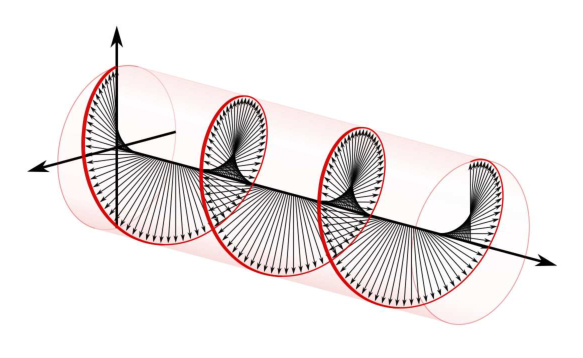
\includegraphics[width=\columnwidth]{modules/m0131_Circular.Polarization.Circularly.Polarized.Light_Without.Components_Right.Handed.eps}\end{center} 
% https://en.wikipedia.org/wiki/File:Circular.Polarization.Circularly.Polarized.Light_Without.Components_Left.Handed.svg
\centerline{\scriptsize 
by~\hyperref[m0131_Circular.Polarization.Circularly.Polarized.Light_Without.Components_Credit]{Dave3457} 
} 
\caption{
\label{m0131_fLCP-RCP}
Left-circular polarization (LCP; top) and right-circular polarization (RCP; bottom).
}
\end{figure}

%ORB HIGHLIGHT
\begin{mdframed}[backgroundcolor=yellow!20,nobreak=true] 
A wave is said to exhibit circular polarization if the electric field vector rotates with constant magnitude.  Left- and right-circular polarizations may be identified by the direction of rotation with respect to the direction of propagation. 
\end{mdframed}

In engineering applications, circular polarization is useful when the relative orientations of transmit and receive equipment is variable and/or when the medium is able rotate the electric field vector.  For example, radio communications involving satellites in non-geosynchronous orbits typically employ circular polarization.
In particular, satellites of the U.S. Global Positioning System (GPS) 
\index{Global Positioning System (GPS)}
transmit circular polarization because of the variable geometry of the space-to-earth radio link and the tendency of the Earth's ionosphere to rotate the electric field vector through a mechanism known \emph{Faraday rotation} 
\index{Faraday rotation}
(sometimes called the ``Faraday effect'').
If GPS were instead to transmit using a linear polarization, then a receiver would need to continuously adjust the orientation of its antenna in order to optimally receive the signal.   
Circularly-polarized radio waves can be generated (or received) using pairs of perpendicularly-oriented dipoles that are fed the same signal but with a $90^{\circ}$ phase shift, or alternatively by using an antenna that is intrinsically circularly-polarized, such as a helical antenna 
\index{antenna!helical}
(see ``Additional Reading'' at the end of this section). 

Linear and circular polarization are certainly not the only possibilities.
\emph{Elliptical polarization} 
\index{polarization!elliptical}
results when $E_x$ and $E_y$ do not have equal magnitude.
Elliptical polarization is typically not an intended condition, but rather is most commonly observed as a degradation in a system that is nominally linearly- or circularly-polarized.  For example, most antennas that are said to be ``circularly polarized'' instead produce circular polarization only in one direction and various degrees of elliptical polarization in all other directions.   

{\bf Additional Reading:}
\begin{itemize}
\item ``\href{https://en.wikipedia.org/wiki/Polarization_(waves)}{Polarization (waves)}'' on Wikipedia.
\item ``\href{https://en.wikipedia.org/wiki/Dipole_antenna}{Dipole antenna}'' on Wikipedia.
\item ``\href{https://en.wikipedia.org/wiki/Polarizer}{Polarizer}'' on Wikipedia.
\item ``\href{https://en.wikipedia.org/wiki/Faraday_effect}{Faraday effect}'' on Wikipedia.
\item ``\href{https://en.wikipedia.org/wiki/Helical_antenna}{Helical antenna}'' on Wikipedia.
\end{itemize}

\index{waves!polarization|)}
